\documentclass{beamer}
\usepackage{ragged2e}  %package for justification
\begin{document}
\section{Message Passing}

\subsection{Introduction}
\begin{frame}
	\centering
	\large Unit-II\\
	\huge Message Passing
\end{frame}


\begin{frame}
	\frametitle{Introduction}
		Two basic methods for for information sharing as as follows
		\begin{enumerate}
		\item Shared Data Approach\\
		\begin{figure}
			\centering
			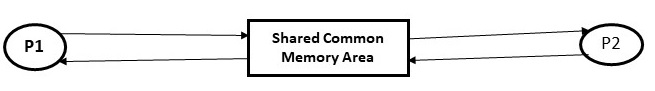
\includegraphics[width=10cm]{sharedDataApproach.jpg}\\
			\caption{Shared Data Approach}
		\end{figure}
		\item Message Passing Approach\\
		\begin{figure}
			\centering
			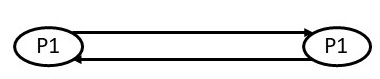
\includegraphics[width=10cm]{messagePassingApproach.jpg}
			\caption{Message Passing Approach}
		\end{figure}
		\end{enumerate}
\end{frame}

\subsection{Features of MPS}
\begin{frame}
	\frametitle{Desirable Features of a good Message Passing System}
	\begin{enumerate}
		\item Simplicity
		\item Uniform Semantics
		\begin{itemize}
			\item Local Communication
			\item Remote Communication
		\end{itemize}
		\item Efficiency
		\item Reliability
		\item Correctness\\
			Issues related to correctness are
		\begin{itemize}
			\item Atomicity
			\item Ordered Delivery
			\item Survivability
		\end{itemize}
		\item Flexibility
		\item Security
		\item Portability
	\end{enumerate}
\end{frame}


\subsection{Issues}
\begin{frame}[allowframebreaks]
	\frametitle{Issues in IPC by Message Passing}
	\justifying{A message is a block of information formatted by a sending process in such a manner that it is meaningful to the receiving process.\\
	In the designing of an IPC protocol for message-passing system, the following important issues need to be considered.}
	\begin{figure}
		\centering
		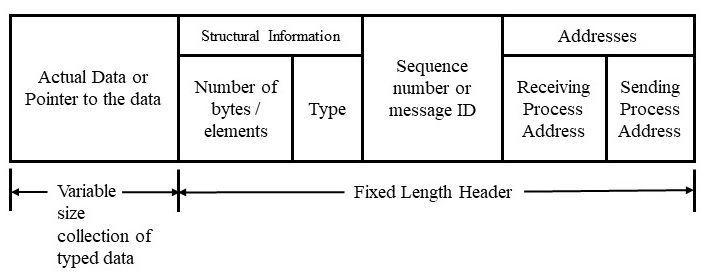
\includegraphics[width=10cm]{messageStructure.jpg}
		\caption{A Typical Message Structure}
	\end{figure}
	\framebreak
	In designing of an IPC for MPS, the following important issues need to be considered:
	\begin{enumerate}
		\item Who is the sender?
		\item who is the receiver?
		\item Is there one receiver or many receivers?
		\item Is the message guaranted to have been accepted by its receiver?
		\item Does the sender need to wait for a reply?
		\item What should be done is a catastrophic event such as a node crash of a communication link failure occurs during the course of communication?
		\item What should be done if the receiver is not ready to accept the message:Will the message be discarded or stored in a buffer? In case of buffering,what shoul be done if athe buffer is full?
		\item is there are several outstanding messages for a receiver, can it choose the order in which to service the outstanding messages?
	\end{enumerate}	 
\end{frame}


\subsection{Synchronization}
\begin{frame}[allowframebreaks]
	\frametitle{Synchronization}
	A central issue in the communication structure is the synchronization. The semantics    
	used synchronization may be broadly classified as
	\begin{itemize}
		\item Blocking
		\item Non-Blocking
	\end{itemize}
	When both the send and receive primitives of a communication between two processes use 
	blocking semantics, the communication is said to be synchronous; otherwise it is 
	asynchronous.
	\vspace{2cm}
	\framebreak
	\begin{figure}
		\centering
		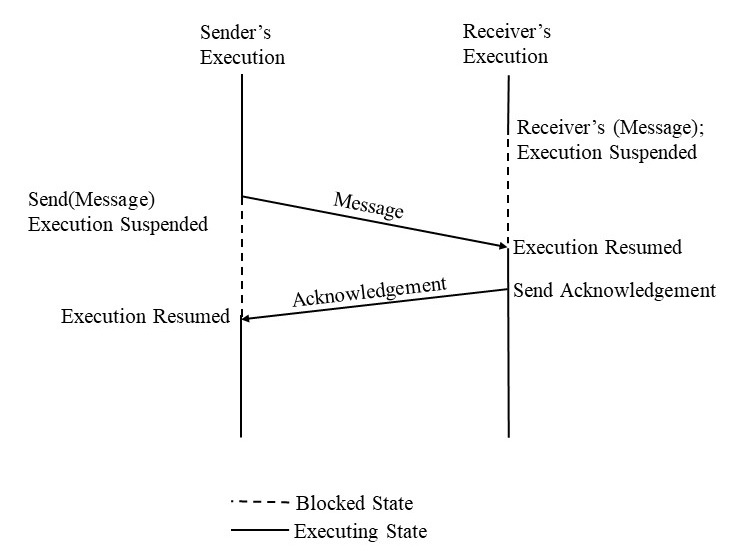
\includegraphics[width=9cm]{synchronousMode.jpg}
		\caption{Synchronous Mode of Communication with send and receive primitives having 
		blocking type semantics.}
	\end{figure}
\end{frame}


\subsection{Buffering}
\begin{frame}[allowframebreaks]
	\frametitle{Buffering}
	The synchronous and asunchronous mode of communication correspond respectively to the 
	two extremes of buffering: a Null Buffer or No Buffering and a buffer with unbounded 
	capacity. Other two commonly used buffering strategies are Single-buffering and finite 
	bound or multiple message buffers. These four types of buffering strategies are;
	\begin{itemize}
		\item Null Buffer or No Buffering
		\item Single Message Buffer
		\item Unbounded-Capacity Buffer
		\item Finite Bound or Multiple Message Buffer
	\end{itemize}
	\vspace{1.5cm}		
	\framebreak
	\begin{figure}
		\centering
		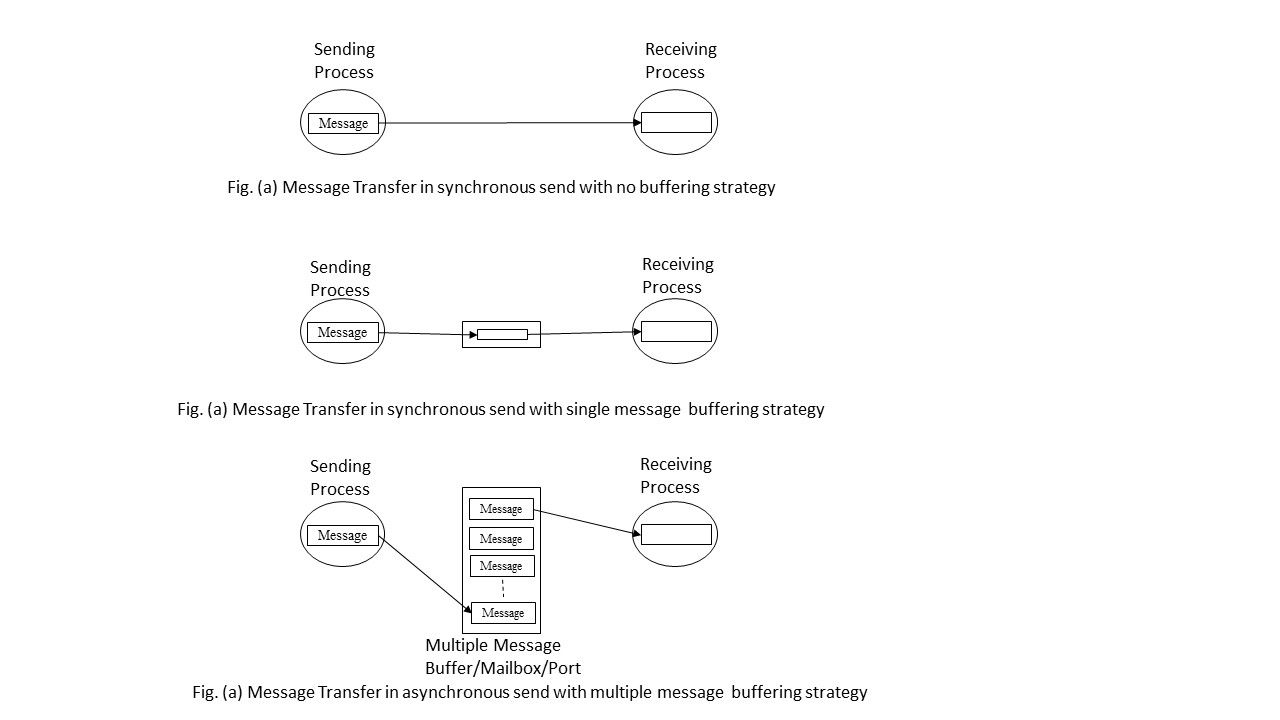
\includegraphics[width=15cm]{buffering.jpg}
	\end{figure}
	\vspace{1cm}
\end{frame}



\subsection{Multidatagram}
\begin{frame}
	\frametitle{Multidatagram Messages}
	\begin{itemize}
		\item Datagram
		\item MTU
		\item Single Datagram Messages
		\item Multi Datagram Messages
	\end{itemize}
	\vspace{4cm}
\end{frame}


\subsection{Encoding & Decoding}
\begin{frame}
	\frametitle{Encoding and Decoding of Message Data}
	
\end{frame}









\end{document}